\section{Problem Statement}
\label{sec:problem_statement}

In this section, the problem we focus on in this paper and our insight will be presented, respectively. 

The road network of a transport system is characterized as a directed graph $G = (V, E, A)$, where a set of $N = |V|$ vertices $V$ denote the traffic nodes (e.g., sensors deployed in the traffic network); a set of edges $E$ depict the connectivity among nodes; and the adjacency matrix $A \in \mathbb{R}^{N \times N}$ describes the connectivity in the network, where $A_{u,v}=1$ refers to a connection between node $u$ and node $v$, otherwise zero.

\begin{figure*}[!ht]
    \centering
    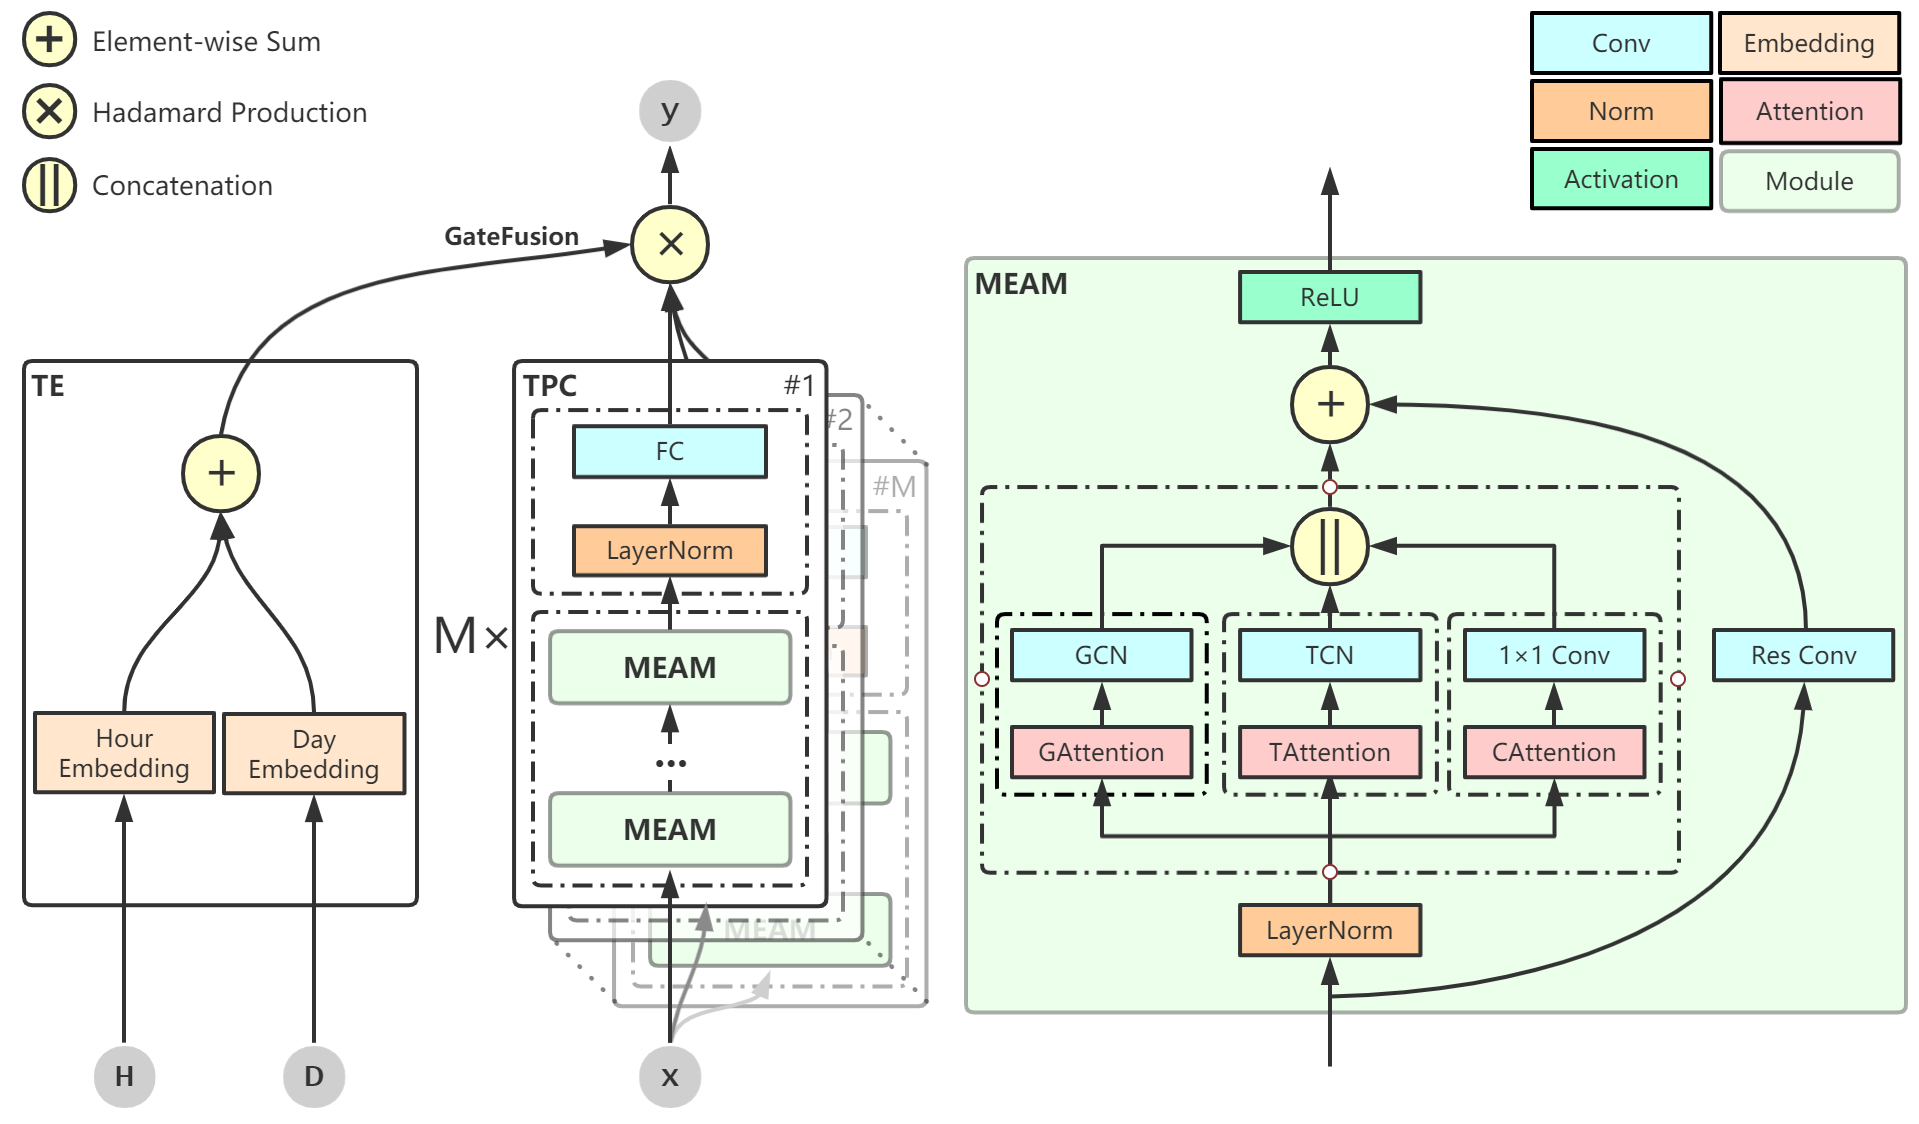
\includegraphics[width=0.64\textwidth]{pictures/Framework.png}
    \caption{An overview of the proposed MS-GAT to model multi-aspect traffic signal couplings. Left: Architecture of MS-GAT, which adopts the multi-component structure with time-gated fusion. Right: Core module of MS-GAT, i.e., multi-relational embedding abreast module (MEAM), which implements the interaction decoupling and multi-relational couplings respectively at its two ends by our multi-dimensional attention mechanism, while learning the embeddings of spatial relations, temporal relations and channel relations in a synchronously handling manner.}
    \label{fig:framework}
\end{figure*}

In a traffic network, all traffic conditions $X$ describe the status of the network. These traffic conditions are multivariate, corresponding to various traffic signals such as traffic volume, density and speed. Suppose there are $d_c$ types of available traffic signals (or indicators), each traffic signal is treated as a separate information channel of traffic nodes, similar to the concept of image channel in computer vision. We then have $X=\left < X(1),\dots,X(d_c) \right >$, where each term $X(l)$ (here, $1 \leq l \leq d_c$) is a random variable to depict a traffic condition, e.g., the observations (or measurement) of traffic flow. The multivariate observations at each traffic node capture the all-channel information of that node, which is called a node’s \textit{channel dimension}. The graph corresponding to the entire traffic network is represented by the interactions between all random variables (from $X(1)$ to $X(d_c)$), which is called the \textit{channel relation} over all $d_c$ channels in the network. 
In a road network, the traffic conditions may change over time, forming a dynamic graph. Assume there are $t_p$ time steps, the traffic conditions $X$ are composed of a sequence of $t_p$ temporal random graph snapshots (each graph snapshot $X^{t}$ corresponds to the traffic network profile at a time point $t$), i.e., $X = [X^{t_1}, \dots , X^{t_p}]$. This time series describe the traffic conditions in terms of a \textit{temporal dimension} of traffic nodes, and the interdependence between time-specific traffic conditions (i.e., different graph snapshots $X^t$ and $X^{t^{'}}$, here $t_1 \leq t, t^{'} \leq t_p$) along the temporal dimension forms the \textit{temporal correlation}  in the network. 
Further, each node of the network is affiliated with multiple channels of signals, and each signal is temporal. Hence, the overall traffic conditions $X$ can also be viewed as a set of $N$ node-oriented random variables, i.e., $X = \left\{X_1, \dots , X_N\right\}$, where each variable $X_v$ denotes the traffic conditions of the node $v$, forming the \textit{spatial dimension} of a node. The interdependence between node-specific variables captures the \textit{spatial correlation} between nodes in the network.  

Accordingly, we can model a traffic network in terms of channel, temporal and spatial dimensions, which offers a three-dimensional view of a traffic system. Then any node $v$ can be modeled by a three-dimensional vector $X_v^{t}(l)$ with its $l^{th}$ signal at time point $t$. The three dimensions further capture various traffic conditions (signals). In addition, the joint modeling of their temporal, spatial and spatio-temporal relations provide a deep quantification of a complex traffic network. 

Consequently, the GNN representation of a traffic network maps a physical system with various traffic signals to a graph $G$ with nodes $\left\{X_v^{t}(l)\right\}$ over $t_p$ time steps. The problem of this GNN-based traffic prediction is to learn a mapping network $f_G$ between the $t_p$ steps of historical traffic conditions $X = [X^1,\dots, X^{t_p}]$ and the next $t_q$ steps of traffic conditions $\hat{X} = [X^{t_p + 1},\dots, X^{t_p + t_q}]$ in the graph $G$.

\begin{equation}
    [X^{t_p + 1}, \dots , X^{t_p + t_q}] = f_G(X^1, \dots, X^{t_p};\theta)
    \label{eqn:target_function}
\end{equation}

where $\theta$ stands for the learnable parameters of graph $G$.

\textbf{Our insight.} The above problem statement formulates a traffic system as a coupled traffic network where diverse traffic signals (e.g., from multiple sensors) are coupled with each other, which differs from the existing assumptions and methods. Figure~\ref{fig:core} illustrates the framework of modeling spatio-temporal traffic signal couplings in a dynamic coupled traffic network with various channels and nodes by a multi-relational graph. Our model extracts the channels of traffic signals, temporal signal development, and interactions between signals at each node, between nodes and over time. We further decouple them by representing their temporal relations, spatial relations, and channel relations. The multi-relational representations are then coupled to build the multi-relational view of a dynamic traffic network. Consequently, the construction of multivariate time series of interactive traffic signals in a traffic system integrates various traffic signals and their multi-aspect relations. We expand GNNs to represent this multi-dimensional and multi-relational view, which shows a more powerful capability of capturing much richer multivariate observations and their hidden spatio-temporal relations in a traffic system than the existing methods.

